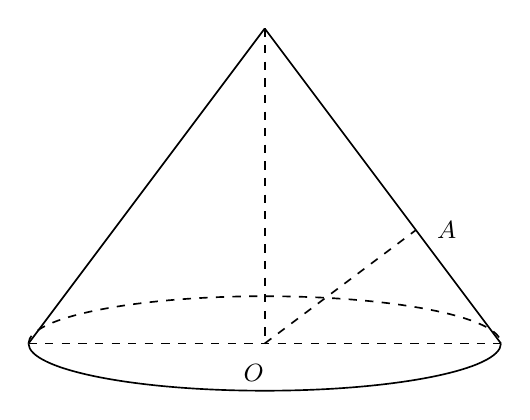
\begin{tikzpicture}[line width=0.6pt, font=\small]
\coordinate (V) at (0,4);
\coordinate (O) at (0,0);
\coordinate (L) at (-3,0);
\coordinate (R) at (3,0);
\coordinate (A) at (1.92,1.44);
% base ellipse: front solid, back dashed
\draw (L) arc[start angle=180, end angle=360, x radius=3, y radius=0.6];
\draw[dashed] (L) arc[start angle=180, end angle=0, x radius=3, y radius=0.6];
% diameter and axis
\draw[dashed] (L) -- (R);
\draw[dashed] (V) -- (O);
% generatrices
\draw (V) -- (L);
\draw (V) -- (R);
% OA
\draw[dashed] (O) -- (A);
% labels with clearance
\node[below, xshift=-4pt, yshift=-4pt] at (O) {$O$};
\node[right, xshift=4pt] at (A) {$A$};
\end{tikzpicture}